\documentclass{../../Proposal/LaTeX-proposal/deliverablereport}
\usepackage[style=alphabetic,backend=biber]{biblatex}
\addbibresource{../../lib/kbibs/kwarc.bib}
\addbibresource{../../lib/deliverables.bib}
\addbibresource{rest.bib}
% temporary fix due to http://tex.stackexchange.com/questions/311426/bibliography-error-use-of-blxbblverbaddi-doesnt-match-its-definition-ve
\makeatletter\def\blx@maxline{77}\makeatother

% TIkZ magic
\usepackage{tikz,standalone}
\usetikzlibrary{backgrounds,shapes,fit,shadows}
\makeatletter%%%%%%%%%%%%%%%%%%%%%%%%%%%%%%%%%%%%%%%%%%%%%%%%%%%%%%%%%%%%%%%%%
% A TIKZ library for MMT Theory Graphs
% copyright 2014 Michael Kohlhase; Released under the LPPL
%%%%%%%%%%%%%%%%%%%%%%%%%%%%%%%%%%%%%%%%%%%%%%%%%%%%%%%%%%%%%%%%%
%
% this library provides some standardized node and arrow styles for formatting MMT graph
% diagrams in tikz. The advantage is that we can classify the arrows and nodes
% symbolically and with the styles in this library achieve a uniform look that helps
% readability. 
%
%%%%%%%%%%%%%%%%%%%%%%%%%%%%%%%%%%%%%%%%%%%%%%%%%%%%%%%%%%%%%%%%%

%%% 1. Theories
% a generic theory
\def\outerthysep{.3mm}
\def\innerthysep{.5mm}
\tikzstyle{thy}=[draw,outer sep=\outerthysep,rounded corners,inner sep=\innerthysep]
% a primitive theory
\tikzstyle{primthy}=[thy,double]
% a theory graph 
\tikzstyle{thygraph}=[draw,outer sep=1mm,rounded corners,dashed]

%%% 2. Arrows 
%%% 2.1. Arrowtips (only internal)
\usetikzlibrary{arrows}
\newcommand{\@mmtarrowtip}{angle 45}
\newcommand{\@mmtreversearrowtip}{angle 45 reversed}
\newcommand{\@mmtarrowtipepi}{triangle 45}
\newcommand{\@mmtarrowtipmonoright}{right hook}
\newcommand{\@mmtarrowtipmonoleft}{left hook}
\newcommand{\@mmtarrowtippartial}{right to}
\newcommand{\@mmtarrowtippartialleft}{left to}
\newcommand{\@mmtreversearrowtippartial}{right to reversed}
\newcommand{\@mmtreversearrowtippartialleft}{left to reversed}

%%% 2.2 the arrow sstyles in graphs
\usetikzlibrary{decorations,decorations.pathmorphing,decorations.markings}
% any morphism 
\tikzstyle{morph}=[-\@mmtarrowtip,thick] 
\tikzstyle{mapsto}=[|-\@mmtarrowtip] %| any morphism 
% structures
\tikzstyle{struct}=[-\@mmtarrowtip,thick]
% inclusions: regular, partial, and left variants
\tikzstyle{include}=[\@mmtarrowtipmonoright-\@mmtarrowtip,thick]
\tikzstyle{revinclude}=[\@mmtarrowtip-\@mmtarrowtipmonoright,thick]
\tikzstyle{pinclude}=[\@mmtarrowtipmonoright-\@mmtarrowtippartial,thick]
\tikzstyle{includeleft}=[\@mmtarrowtipmonoleft-\@mmtarrowtip,thick]
\tikzstyle{pincludeleft}=[\@mmtarrowtipmonoleft-\@mmtarrowtippartialleft,thick]
% views: regular, mono, partial, and left variants
\tikzstyle{preview}=[decorate,
                                decoration={coil,aspect=0,amplitude=1pt,
                                                    segment length=6pt,
                                                    pre=lineto,pre length=3pt,
                                                    post=lineto,post length=5pt},
                                thick]
\tikzstyle{view}=[preview,-\@mmtarrowtip]
\tikzstyle{mview}=[preview,\@mmtarrowtipmonoright-\@mmtarrowtip]
\tikzstyle{pview}=[preview,-\@mmtarrowtippartial]
\tikzstyle{pmview}=[preview,\@mmtarrowtipmonoright-\@mmtarrowtippartial]
\tikzstyle{viewleft}=[preview,-\@mmtarrowtip]
\tikzstyle{mviewleft}=[preview,\@mmtarrowtipmonoleft-\@mmtarrowtip]
\tikzstyle{pviewleft}=[preview,-\@mmtarrowtippartialleft]
\tikzstyle{pmviewleft}=[preview,\@mmtarrowtipmonoleft-\@mmtarrowtippartialleft]
\tikzstyle{adoption}=[preview,thin,double,-\@mmtarrowtip]
% biviews: regular, partial, and left variants
\tikzstyle{biview}=[preview,\@mmtarrowtip-\@mmtarrowtip]
\tikzstyle{pbiview}=[preview,\@mmtreversearrowtippartial-\@mmtarrowtippartial]
\tikzstyle{pbiviewleft}=[preview,\@mmtreversearrowtippartialleft-\@mmtarrowtippartialleft]
% defining views (experimental)
\tikzstyle{defview}=[preview,densely dotted,-\@mmtarrowtip]
% meta-theory inclusion
\tikzstyle{meta}=[dotted,-\@mmtarrowtip,thick]
% conservative extensions (abbreviation)
\tikzstyle{conservative}=[hooks-\@mmtarrowtip,double] 
% conservative development
\tikzstyle{conservdev}=[hooks-\@mmtarrowtip,dashed,double] 

% antimorphisms as striktthroughs
\tikzset{anti/.style={
    decoration={markings, mark=between positions 0.2 and 0.8 step 4mm with {
        \draw [thick,-] ++ (-3pt,-3pt) -- (3pt,3pt);}},
    postaction={decorate}}}

% parallel markup
\tikzstyle{parallel}=[\@mmtarrowtip-\@mmtarrowtip,dashed]

%%%% 3. Realms 
\tikzstyle{prerealm}=[draw=blue!40,rectangle,rounded corners,inner sep=10pt,inner ysep=20pt]
\tikzstyle{realm}=[prerealm,fill=gray!4]
\tikzstyle{pillar}=[prerealm,fill=gray!10]

%%% 4. convenience macros
%%% 4.1 the \mmtthy macro takes three arguments, name, decl, axioms and makes a 
% table-like structure
\newcommand\mmtthy[3]{\def\@second{#2}\def\@third{#3}%
\begin{array}{l}\textsf{#1}%
\ifx\@second\@empty\else\\\hline #2\fi%
\ifx\@third\@empty\else\\\hline #3\fi%
\end{array}}
%%% 4.2 the \mmtar takes two arguments, some tikz options, and an arrow style. \nmmtar
% is a variant that also has a name on top.
\newcommand\mmtar[2][]{\raisebox{.5ex}{\tikz[#1]{\draw[#2] (0,0) -- (.6,0);}}}
\newcommand\nmmtar[3][]{\raisebox{.4ex}{\tikz[#1]{\draw[#2] (0,0) --
      node[above]{\ensuremath{\scriptstyle #3}} (.8,0);}}}
%%%% 3.3 Pushout symbols
%%  (after http://tex.stackexchange.com/questions/1144/pushouts-and-pullbacks)
%% \nepushout[<pos>]{<basenode>}{<targetnode>} positions a pushout symbol 
%% (available separately as \pushoutsymb) <pos> of the way between <basenode>
%%  and <targetnode>. 
\usetikzlibrary{calc}
\newcommand\@pushout[4][]{\def\@test{#1}%
\ifx\@test\@empty\def\@@num{.5}\else\def\@@num{#1}\fi%
\begin{scope}[shift=($(#2)!\@@num!(#3)$)]\@nameuse{@#4pushoutsymb}\end{scope}} 
\newcommand\@nepushoutsymb{\draw +(-.2,0) -- +(0,0)  -- +(0,-.2);\fill +(-.1,-.1) circle (.03);}
\newcommand\nepushoutsymb{\tikz{\@nepushoutsymb}}
\newcommand\nepushout[3][]{\@pushout[#1]{#2}{#3}{ne}}

\newcommand\@sepushoutsymb{\draw +(-.2,0) -- +(0,0)  -- +(0,.2);\fill +(-.1,.1) circle (.03);}
\newcommand\sepushoutsymb{\tikz{\@sepushoutsymb}}
\newcommand\sepushout[3][]{\@pushout[#1]{#2}{#3}{se}}

\newcommand\@nwpushoutsymb{\draw +(.2,0) -- +(0,0)  -- +(0,-.2);\fill +(.1,-.1) circle (.03);}
\newcommand\nwpushoutsymb{\tikz{\@nwpushoutsymb}}
\newcommand\nwpushout[3][]{\@pushout[#1]{#2}{#3}{nw}}

\newcommand\@swpushoutsymb{\draw +(.2,0) -- +(0,0)  -- +(0,.2);\fill +(.1,.1) circle (.03);}
\newcommand\swpushoutsymb{\tikz{\@swpushoutsymb}}
\newcommand\swpushout[3][]{\@pushout[#1]{#2}{#3}{sw}}

\newcommand\@npushoutsymb{\draw +(-.1,-.1) -- +(0,0)  -- +(.1,-.1);\fill +(0,-.1) circle (.03);}
\newcommand\npushoutsymb{\tikz{\@npushoutsymb}}
\newcommand\npushout[3][]{\@pushout[#1]{#2}{#3}{n}}

\newcommand\@spushoutsymb{\draw +(-.1,.1) -- +(0,0)  -- +(.1,.1);\fill +(0,.1) circle (.03);}
\newcommand\spushoutsymb{\tikz{\@spushoutsymb}}
\newcommand\spushout[3][]{\@pushout[#1]{#2}{#3}{s}}

\newcommand\@wpushoutsymb{\draw +(-.1,-.1) -- +(0,0)  -- +(-.1,.1);\fill +(-.1,0) circle (.03);}
\newcommand\wpushoutsymb{\tikz{\@wpushoutsymb}}
\newcommand\wpushout[3][]{\@pushout[#1]{#2}{#3}{w}}

\newcommand\@epushoutsymb{\draw +(.1,.1) -- +(0,0)  -- +(.1,-.1);\fill +(.1,0) circle (.03);}
\newcommand\epushoutsymb{\tikz{\@epushoutsymb}}
\newcommand\epushout[3][]{\@pushout[#1]{#2}{#3}{e}}

%%%%%% testing them: 
% \begin{tikzpicture}[scale=1.5]
%   \node (a) at (0,0) {a};
%   \node (b) at (1,0) {b};
%   \node (c) at (1,1) {c};
%   \node (d) at (0,1) {d};
%   \nepushout[.8]{a}c;
%   \nwpushout[.8]{b}d;
%   \sepushout[.8]{d}b;
%   \swpushout[.8]{c}a;
%   \draw (a) -- (b) -- (c) -- (d) -- (a);
%   \node (aa) at (4,0) {a};
%   \node (bb) at (3.5,.5) {b};
%   \node (cc) at (4,1) {c};
%   \node (dd) at (4.5,.5) {d};
%   \draw (aa) -- (bb) -- (cc) -- (dd) -- (aa);
%   \npushout[.8]{aa}{cc};
%   \spushout[.8]{cc}{aa};
%   \wpushout[.8]{bb}{dd};
%   \epushout[.8]{dd}{bb};
% \end{tikzpicture}

%%% Local Variables:
%%% mode: latex
%%% TeX-master: "test"
%%% End:
\makeatother

\usepackage{standalone}
\usepackage[show]{ed}

\usepackage{graphicx}
\usepackage{float}

\usepackage{color}
\definecolor{gray}{rgb}{0.4,0.4,0.4}
\definecolor{darkblue}{rgb}{0.0,0.0,0.6}
\definecolor{cyan}{rgb}{0.0,0.6,0.6}

\hypersetup{colorlinks}

\deliverable{dksbases}{design}
\issue{136}
\deliverydate{31/08/2016}
\duedate{31/08/2016 (Month 12)}
\def\pn{OpenDreamKit\xspace}

\author{Michael Kohlhase, Florian Rabe, Tom Wiesing, Paul-Olivier Dehaye, Dennis M\"uller}

\usepackage[parfill]{parskip}

% for definitions
\usepackage{amsthm}
\newtheorem{mydef}{Definition}

\usepackage{xspace}

%%%%%%%% fix %%%%%%%%%%%
\makeatletter\gdef\deliv@lead{JU}\makeatother
%%%%%%%% endfix %%%%%%%%%%%


% Keep all these presented in a standard fashion
\newcommand{\SageMath}{SageMath\xspace}
\newcommand{\GAP}{GAP\xspace}
\newcommand{\LMFDB}{LMFDB\xspace}
\newcommand{\OEIS}{OEIS\xspace}
\newcommand{\python}{Python\xspace}
\newcommand{\MMT}{MMT\xspace}
\newcommand{\FindStat}{FindStat\xspace}
\newcommand{\Pari}{Pari\xspace}
\newcommand{\PariGP}{Pari/GP\xspace}

\newcommand{\Magma}{Magma\xspace}

\newcommand{\DKS}{$\mathcal{DKS}$}

\begin{document}


\begin{abstract}
  To build Virtual Research environments (VREs) we need to integrate three different aspects, Data (D), Knowledge (K) and Systems (S). We want to achieve this using the well-established framework of theory graphs. In this setting we need to expand the current model of theories.

  In this report we present the design process towards \textit{DKS} theories including the overall architecture, a survey of the systems involved, our current implementation of \textit{DK} theories as well as our plans for the future.
\end{abstract}
\maketitle 


\newpage\tableofcontents\newpage

\section{Introduction}\label{sec:intro}

\begin{newpart}{MK: adapted from Tom's Thesis}
There is a large and vibrant ecosystem of open-source mathematical software systems.
These systems can range from calculators, which are only capable of performing simple
computations, via mathematical databases (curating collections of a mathematical objects)
to powerful modeling tools and computer algebra systems (CAS). 

Most of these systems are very specific -- they focus on one or very few aspects of
mathematics.  For example, the ``Online Encyclopedia of Integer Sequences''
(OEIS~\cite{Sloane:oeis12,oeis}) focuses on sequences over $\mathbb{Z}$ an their
properties and the ``L-Functions and Modular Forms Database''
(LMFDB)~\cite{Cremona:LMFDB16,lmfdb:on} objects in number theory pertaining to Langland's
program.  GAP~\cite{GAP:on} excels at discrete algebra, whereas
SageMath~\cite{SageMath:on} focuses on Algebra and Geometry in general, and
Singular~\cite{singular:on} on polynomial computations, with special emphasis on
commutative and non-commutative algebra, algebraic geometry, and singularity theory.

For a mathematician however (a user; let us call her Jane) the systems themselves are not relevant, instead she only cares about being able to solve problems. 
Typically, it is not possible to solve a mathematical problem using only a single program. 
Thus Jane needs to work with multiple systems and combine the results to reach a solution. 
Currently there is very little help with this practice, so Jane has to isolate sub-problems the respective systems are amenable to, formulate them into the respective input language, collect results, and reformulate them for the next system a tedious and error-prone process at best, a significant impediment to scientific progress in its overall effect. 
Solutions for some situations certainly exist, which can help get Jane unstuck, but these are ad-hoc and for specific, often-used system combinations only. 
Each of these requires a lot of maintenance and does not scale to a larger set of specialist systems. 

The OpenDreamKit project, which aims at a mathematical VRE toolkit, proposes the Math-in-the-Middle (MitM~\cite{DehKohKon:iop16}) Paradigm, an interoperability framework based on a flexiformal
representation of mathematical knowledge and aligns this with system-generated interface
theories. 

In this paper we instantiate the MitM paradigm with a concrete domain development and
evaluate it on a distributed computing GAP, SageMath and Singular.\ednote{ we generally we
  want to show that the promises in the CICM paper become reality.}

We will use the following example as a running example: Jane wants to act on singular
polynomials with GAP permutation groups\ednote{MK@(MP|VA): }

 \ednote{MK: continue with the structure} 
\end{newpart}

%%% Local Variables:
%%% mode: latex
%%% TeX-master: "paper"
%%% End:

\section{Report and Case-Study}\label{sec:survey}
\ednote{@Paul: give a general overview of the results of the case-study}

%%% Local Variables:
%%% mode: latex
%%% TeX-master: "report"
%%% End:


\section{Theory Graphs: The Knowledge Aspect}\label{sec:MMT}
 We only sketch \MMT here to the extent that we need it and refer to \cite{RabKoh:WSMSML13} for details.
An OMDoc/MMT theory graph is a diagram in the category of \MMT theories and theory morphisms.
Theories represent all kinds of languages such as mathematical foundations and type systems as well as individual mathematical theories.
Theory morphisms represent relations between them including translations, imports, and representation theorems.

\paragraph{Theories}
In the simplest case (which is sufficient for our purposes here) an \MMT \textbf{theory} is a set of symbol declarations.
Each \textbf{symbol declaration} must have a name and may optionally have a type object, a defining object, and arbitrary meta-data (such as tags, cross-references, comments, etc).
The \textbf{objects} are OpenMath 2.0 objects \cite{BusCapCar:2oms04} --- these are complex expressions formed from application, binding, variables, literals, and symbol references.
\ednote{@TW: give example of a theory, e.g., a fragment of the ODK math theory}

Critically, \MMT enforces structural validity: Every object may only reference symbols that are declared in or imported into the containing theory.
But \MMT abstracts from the foundational semantics such as type and logic systems that specify exactly which objects are meaningful.
This puts \MMT into a powerful intermediate position, where enough structure is guaranteed for knowledge management while not committing to a particular foundation.

Above we have skipped the \MMT module system, which is not essential for our results here.
However, one detail of the \MMT module system \emph{is} critical: Every theory may have a \textbf{meta-theory}.
Practically, the meta-theory mostly behaves like a plain import.
But conceptually, the meta-theory of a theory $T$ is the language that provides the foundational background to understand $T$.
The most common use case employs three meta-levels: Firstly, an \MMT theory introduces a logical framework $F$.
Secondly, $F$ serves as the meta-theory of a foundation $L$, which uses the symbols of $F$ to define a particular type system and logic.
Thirdly, a library of mathematical knowledge is developed as a theory graph in which all theories have meta-theory $L$.
\ednote{@TW: give example graph involving some theories involved in this report}

Most systems (including most systems involved in \pn) focus on the third level only.
The second level is usually left implicit, e.g., because it is hard-coded in the implementation of computation system.
And because the second level is hard-coded, there is no need for the first level.
For system integration, it is important to make the second level explicit so that the semantics of the exchanged knowledge can be specified.
Thus, \MMT already anticipates much of the high-level concepts needed for the system-spanning \DKS-bases in \pn.

\paragraph{Theory Morphisms}
There are two kinds of theory morphisms: imports and views.
Imports are the central for building theories modularly by pulling together symbols introduced in other theories.
Practically, imports can be seen amount to copying symbol declarations while instantiating, renaming, or otherwise modifying them.
The semantics of theories with imports is defined via colimits.

A view from theory $S$ to theory $T$, is a translation of $S$-objects to $T$-objects.
Contrary to imports, views are given after the involved theories have been defined.
Thus, they have the character of theorems rather than definitions, and indeed views usually induce proof obligations that must be discharged for a view to be accepted.
In the presence of appropriate logical frameworks, \MMT guarantees a critical property: The translation of objects preserves all properties of the type system and the logic.
In particular, all $S$-theorems are translated to $T$-theorems.

\paragraph{Implementation}
Theory graphs are implemented in the \MMT system~\cite{Rabe:MAGMS13,uniformal:on}.
At its core, this system allows for the declaration of theories along with symbols, imports and views, to build objects and translate them along views.

On top of this, the \MMT system provides a number of logical and knowledge management services.
The former includes computing the respective colimits, translating objects along morphisms, or type checking and proving objects relative to the respective meta-theory.
The latter include import/export of libraries, editing, browsing, and middleware for system integration.
 
\section{Math in the Middle: The Software Aspect}\label{sec:mitm}
  The \pn project intends to integrate multiple mathematical software systems into a VRE
toolkit. These systems are constituted by large collections of algorithms manipulating
highly optimized data structures representing mathematical objects with the intent of
solving specific computational problems. The systems overlap in the mathematical
objects they cover and the problems they can solve, but every system has aspects that are
not covered by any other system (as efficiently or generally). In particular, algorithms,
implementation languages, and data structures differ significantly between systems and are
optimized to their particular domain and intended performance profile. As the systems
represent decades worth of experience and development, a re-implementation is prohibitive
in cost and might lead to systems with greater coverage, but less efficiency.

Given this situation, the integration problem in \pn becomes a problem of establishing an
interoperability layer between systems. As we have seen in the previous section, the
mathematical knowledge -- for specifying the computational problems -- can be expressed
and made interoperable via views in the OMDoc/MMT format, specifying the exact data
structures and intended behavior of software systems -- and possibly verifying that the
implementation conforms to this is the realm of ``Formal Methods''. Again, the effort of
doing this for any of the systems in \pn is prohibitive and way beyond the scope of the
project.

\subsection{Specification of Interfaces}

Fortunately, we do not need implementation-level specification and verification for
integration of existing systems into a VRE toolkit. Specification (of objects and intended
behavior) at the mathematical level is sufficient. In particular quality control
(establishment of correctness of the implementations) can be left to other
means\footnote{In particular, it is independent of interoperability of mathematical
  software systems.} and as a result we can resort to more lightweight methods for
establishing interoperability.

If we analyze mathematical software from a specification-based viewpoint, then we see
three levels: The
\begin{compactenum}[\rm\bf S1.]
\item \textbf{Math Specification} represents the underlying mathematical knowledge and
  the computational problems of our domain.
\item \textbf{Interface Specification} represents the interfaces of mathematical software
  systems: the abstract data structures, and the input/output behavior (and possible
  side-effects) of the user-visible functions and procedures provided by the system.
\item \textbf{Implementation} gives concrete implementations of the interface
  specification in a specific programming language.
\end{compactenum}
Most modern programming languages support the organization of programs into software
libraries by separating the specification (\textbf{S2.}) and implementation levels
(\textbf{S3.}), allowing multiple implementations of a single specification. Examples include
abstract vs. concrete classes in object-oriented programming, signatures vs. structures in
SML, header files vs. C files in C, and operations vs. methods in \GAP. In all of them the
interface specification level is utilized for intra-library interoperability, making use
of the more abstract description of the interface specification that can be instantiated
by its various implementations. The interface specifications usually tie the names of the
interface functions to argument and result types. The specification of intended behavior
is usually left to documentation facilities. This is the domain of the math specification
level (\textbf{S1.}), which is only marginally supported by programming languages, but a
central concern in the \pn project. The math specification level is characterized by some
kind of logical system that can express universal properties like
$\forall x,y. x=\operatorname{sqrt}(y) \Leftrightarrow x^2=y$.

\subsection{The Math-in-the-Middle Paradigm}

In the \pn project we want to cover the software aspect of a math VRE toolkit via an
approach we call ``Math-In-The-Middle'' paradigm (MitM; see~\cite{DehKohKon:iop16} for
details and Figure~\ref{fig:mitm} for an overview diagram). In contrast to most
programming languages MitM paradigm concentrates on levels \textbf{S1.} and \textbf{S2.},
represents them in the OMDoc/MMT format and leaves the implementation (\textbf{S3.}) to
the respective systems.

Here the underlying mathematical knowledge (level \textbf{S1.}), the ``real math'', is
used as a reference ontology (in the ``middle'' -- hence the name) for the math VRE
toolkit. This ontology is represented as an OMDoc/MMT theory graph $M$ as described in the
previous section. For every systen in the \pn VRE toolkit we establish an interface
specification as an OMDoc/MMT theory graph $I$ and link it to the MitM ontology via
\textbf{interface views}. These fulfil two purposes: they align the name spaces of the
systems with the math specification and they specify the intended behavior of the systems
in terms of the MitM ontology: Recall that OMDoc/MMT views transport $I$-theorems to
$M$-theorems, so all properties expressed in these are conserved -- up to the namespace
alignment.

\begin{figure}[ht]\centering
  \def\myxscale{3}\def\myyscale{1.2}
  \documentclass{standalone}
\usepackage[mh]{mikoslides}
% this file defines root path local repository
\defpath{MathHub}{/Users/kohlhase/localmh/MathHub}
\mhcurrentrepos{MiKoMH/talks}
\libinput{WApersons}
% we also set the base URI for the LaTeXML transformation
\baseURI[\MathHub{}]{https://mathhub.info/MiKoMH/talks}

\usetikzlibrary{backgrounds,shapes,fit,shadows,mmt}
\begin{document}
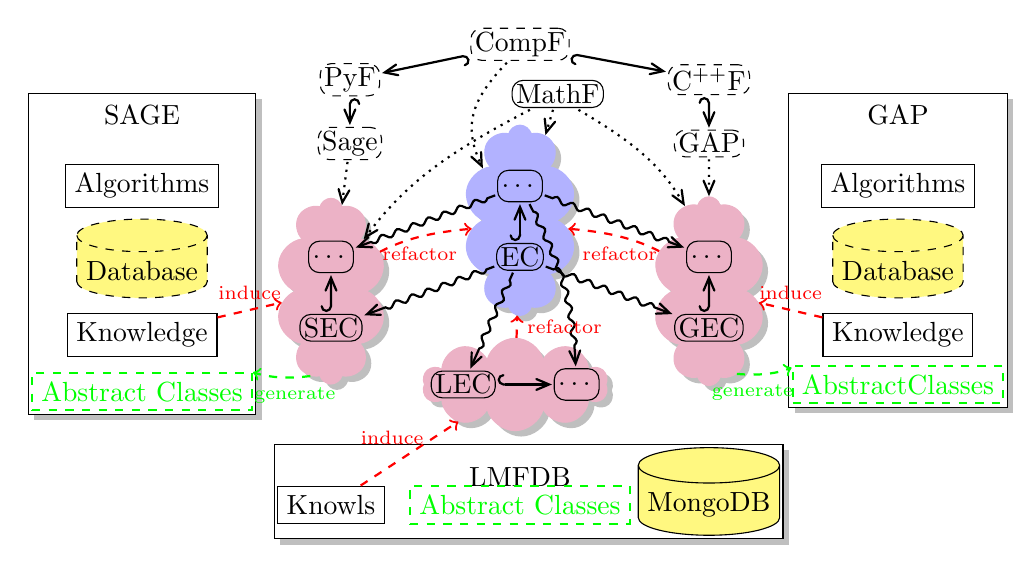
\begin{tikzpicture}[xscale=2.4,yscale=.9]
  \tikzstyle{withshadow}=[draw,drop shadow={opacity=.5},fill=white]
   \tikzstyle{database} = [cylinder,cylinder uses custom fill,
      cylinder body fill=yellow!50,cylinder end fill=yellow!50,
      shape border rotate=90,
      aspect=0.25,draw]
   \tikzstyle{human} = [red,dashed,thick]
   \tikzstyle{machine} = [green,dashed,thick]

\node[thy]  (mf) at (.2,5.3) {MathF};
\node[thy,dashed]  (compf) at (0,6) {CompF};
\node[thy,dashed]  (pf) at (-.9,5.5) {PyF};
\node[thy,dashed]  (cf) at (1,5.5) {C\textsuperscript{++}F};
\node[thy,dashed]  (sf) at (-0.9,4.6) {Sage};
\node[thy,dashed]  (gf) at (1,4.6) {GAP};

\draw[include] (compf) -- (pf);
\draw[includeleft] (compf) -- (cf);
\draw[include] (pf) -- (sf);
\draw[includeleft] (cf) -- (gf);

\node[thy] (kec) at (0,3) {EC};
\node[thy,minimum height=.4cm] (kl) at (0,4) {\ldots};

\node[thy] (sec) at (-1,2) {SEC};
\node[thy,minimum height=.4cm] (sl) at (-1,3) {\ldots};

\node[thy] (gec) at (1,2) {GEC};
\node[thy,minimum height=.4cm] (gl) at (1,3) {\ldots};

\node[thy] (lec) at (-.3,1.2) {LEC};
\node[thy,minimum height=.4cm] (ll) at (.3,1.2) {\ldots};

\node (sc) at (-2,5) {SAGE};
\node[draw] (salg) at (-2,4) {Algorithms};
\node[database,dashed] (sdb) at (-2,2.8) {Database};
\node[draw] (skr) at (-2,1.9) {Knowledge};
\node[draw,machine] (sac) at (-2,1.1) {Abstract Classes};

\node (gc) at (2,5) {GAP};
\node[draw] (galg) at (2,4) {Algorithms};
\node[database,dashed] (gdb) at (2,2.8) {Database};
\node[draw] (gkr) at (2,1.9) {Knowledge};
\node[draw,machine] (gac) at (2,1.2) {AbstractClasses};

\node (lmfdb) at (0,-.1) {LMFDB};
\node[database] (ldb) at (1,-.5) {MongoDB};
\node[draw] (knowls) at (-1,-.5) {Knowls};
\node[draw,machine] (lac) at (0,-.5) {Abstract Classes};

  \begin{pgfonlayer}{background}
    \node[draw,cloud,fit=(sec) (sl),aspect=.4,inner sep=-3pt,withshadow,purple!30] (st) {};
    \node[draw,cloud,fit=(gec) (gl),aspect=.4,inner sep=-4pt,withshadow,purple!30] (gt) {};
    \node[draw,cloud,fit=(kec) (kl),aspect=.4,inner sep=0pt,withshadow,blue!30] (kt) {};
    \node[draw,cloud,fit=(lec) (ll),aspect=3.5,inner sep=-8pt,withshadow,purple!30] (lt) {};
  \end{pgfonlayer}

\begin{pgfonlayer}{background}
  \node[draw,withshadow,fit=(sc) (skr) (sac) (sdb),inner sep=1pt] {};
  \node[draw,withshadow,fit=(gc) (gkr) (gac) (gdb),inner sep=1pt] {};
  \node[draw,withshadow,fit=(lmfdb) (lac) (ldb) (knowls),inner sep=1pt] {};
\end{pgfonlayer}

\draw[view] (kec) -- (sec);
\draw[view] (kec) -- (gec);
\draw[view] (kec) -- (lec);
\draw[include] (kec) -- (kl);
\draw[include] (gec) -- (gl);
\draw[include] (sec) -- (sl);
\draw[include] (lec) -- (ll);
\draw[view] (kl) -- (sl);
\draw[view] (kl) -- (gl);
\draw[view] (kl) to[bend left=5] (ll);

\draw[meta] (mf)  to [bend right=10] (st);
\draw[meta] (sf) -- (st);
\draw[meta] (mf)  to [bend left=10] (gt);
\draw[meta] (gf) -- (gt);
\draw[meta] (mf) -- (kt);
\draw[meta] (compf) to[bend right=15] (kt);

\draw[human,->] (skr) -- node[above]{\scriptsize induce} (st);
\draw[human,->] (gkr) -- node[above]{\scriptsize induce} (gt);
\draw[human,->] (knowls) -- node[left,near end]{\scriptsize induce} (lt);

\draw[machine,->] (gt) to[bend right=30] node[below,near start]{\scriptsize generate} (gac);
\draw[machine,->] (st) to[bend left=30] node[below,near start]{\scriptsize generate} (sac);
\draw[human,->] (st) to[bend left=20] node[below]{\scriptsize refactor} (kt);
\draw[human,->] (gt) to[bend right=20] node[below]{\scriptsize refactor} (kt);
\draw[human,->] (lt) -- node[right]{\scriptsize refactor} (kt);
\end{tikzpicture}
\end{document}
%%% Local Variables: 
%%% mode: latex
%%% TeX-master: t
%%% End: 

  \caption{The MitM paradigm in detail. PyF, C${}^{++}$F and CompF are (basic)
    foundational theories for \python, C${}^{++}$ and a generic computational model. SEC,
    LEC and GEC are theories for \SageMath, \LMFDB and \GAP elliptic curves.}\label{fig:mitm}
\end{figure}

A sketch of the theory graph based on the example of elliptic curves can be
found in Figure~\ref{fig:odk_theories}, an overview of the paradigm can be found
in Figure~\ref{fig:mitm}.  We will not go into details here but show how this
architecture integrates the \emph{Software} and \emph{Knowledge Aspects}.
Clearly, the MitM ontology -- the purple cloud in the middle -- is a
specification of the underlying mathematical knowledge as an OMDoc/MMT theory
graph, while the system interface theories -- the blue clouds around it --
formally specify the names and types (i.e. the argument patterns) and intended
behaviour of the interface functions of the systems (often semi-formally to make
the MitM approach scalable). The OMDoc/MMT views -- the wavy arrows between the
theories -- are interpretation morphisms; in this particular case where they
connect the mathematical specification to the system theories, they express the
``implementation relation''. Thus the OMDoc/MMT framework already allows to
integrate the knowledge and software aspects for system interoperability.

\subsection{Design Decisions and Initial Evaluation}
The MitM paradigm we choose for the software (S) aspect of the \pn VRE toolkit essentially
takes two design decisions:
\begin{compactenum}[\bf D1.]
\item The restriction to formalizing the interface specification (\textbf{S2.}: names and
  types of the interface functions) of the systems is sufficient to ensure system
  interoperability
\item integrating the implementations -- e.g. C\textsuperscript{++} or Python code -- into
  the OMDoc/MMT theories would be overkill here, since the code can only be executed by
  the respective systems -- i.e. \GAP or \SageMath. Therefore we will base our foundation
  on OMDoc/MMT theory graphs directly rather than on an extension of OMDoc/MMT with
  ``biform theories''~\cite{KohManRab:aumftg13,Farmer:btc07} as envisioned in the
  proposal. Biform theories would enable (partial) verification of mathematical software
  systems, but this is not on the critical path towards a mathematical VRE.
\end{compactenum}
The MitM paradigm constitutes a lightweight alternative; identifying and refining it has
been one of the major achievements of the first year in \WPref{dksbases}.

To evaluate the paradigm and the design decisions we have implemented extensions to the
\GAP and \SageMath that export interface theory graphs in the OMDoc/MMT format
(see~Section~\ref{sec:cases} for details):
\begin{compactitem}
\item \GAP exports types, constructors, functions, data, and their documentation: 4097
  Objects exported (2996 unique) in ca. 210 theories.
\item \SageMath exports categories/types, annotates functions: 382 Categories using 25
  Axioms and (in total) 808 methods.
\end{compactitem}
These interface theories allow the representation of all mathematical objects in \GAP and
\SageMath as OpenMath2/MathML3 objects~\cite{BusCapCar:2oms03,CarlisleEd:MathML3} whose
symbols are grounded in the interface theories (interpreted as OpenMath content
dictionaries). \GAP already had an \textbf{OpenMath phrasebook} -- an import/export
facility for OpenMath objects -- and we have developed one for Python and
\SageMath~\cite{py-openmath:on}.

Even though the development of the MitM paradigm is still at an early stage, these case
studies show the potential of the approach. We hope that the nontrivial cost of curating
an ontology of mathematical knowledge and interface views to the interface theories will
be offset by its utility as a resource, which we are currently exploring; the unification
of the knowledge representation components in the \MMT system
\begin{compactenum}
\item enables VRE-wide domain-centered (rather than system-centered) documentation: the
  namespace alignment given by the interface-views allows to re-use documentation for a
  concept, object, or model in the MitM ontology in all interface functions aligned with
  it.
\item can be leveraged for distributed computation via uniform protocols like the
  SCSCP~\cite{HorRoz:ossp09} and MONET-style service
  matching~\cite{CaprottiEtAl:MathServiceMatching04:tr} (the absence of content
  dictionaries -- now given as interface theories -- was the main hurdle that kept these
  from gaining more traction). Again, \GAP already had an SCSCP interface, and we are
  developing one for \SageMath at \cite{py-scscp:on}.
\item will lead to the wider adoption of best practices in mathematical knowledge
  management in the systems involved; in fact, this is already happening: the development
  of the \GAP interface theory exporter led to the discovery of hundreds of documentation
  errors and to a large-scale code refactoring that made type information more explicit
  and could lead to efficiency gains by extended static analysis in the future.
\end{compactenum}

%%% Local Variables:
%%% mode: latex
%%% TeX-master: "report"
%%% End:

%  LocalWords:  pn optimized behavior analyze compactenum textbf organization utilized
%  LocalWords:  characterized forall sqrt Leftrightarrow DehKohKon iop16 mitm centering
%  LocalWords:  myxscale myyscale emph emph formalizing KohManRab aumftg13 btc07 WPref
%  LocalWords:  dksbases compactitem domain-centered ossp09 py-scscp

  
\section{Virtual Theories: The Data Aspect}\label{sec:data}

  \subsection{Virtual Theories}\label{sec:data:def}
  
   OMDoc/MMT theories are limited when it comes to representing large amounts of data.
Conceptually, every database should be represented as one theory, but this can easily lead to very large theories.
For example, the theory for elliptic curves in the \LMFDB would contain \ednote{@TW: add number} symbol declarations: one definition for every curve.
Prior to \pn, \MMT could only load who{e theories into main memory, which made it insufficient as a basis for \DKS-bases.

Moreover, many data-driven theories are technically infinite collections of which only finite fragments have been explored so far.
For example, this applies to all databases in the \LMFDB (each of which enumerates a certain infinite class of mathematical objects) and \OEIS (each of which enumerates a certain integer sequence).
As the explored fragments grow, the set of symbol declarations in the corresponding \MMT theory must grow accordingly.

Therefore, we generalize \MMT theories to allow for a virtual, possibly infinite set of declarations, that is explored dynamically.
The combination of virtual theories with the Math-in-the-Middle approach yields our desired \DKS-bases.

\begin{mydef}[Virtual Theory]
  A \textbf{virtual theory} is like an \MMT theory but with a (possibly infinite) partially ordered set of declarations.
\end{mydef}

We give a trivial example of an infinite virtual theory for the natural numbers:
Besides the usual symbols for $0$ and $\mathtt{succ}$ as well as the Peano axioms, it contains the totally ordered set of one declaration for every natural number.
For example, we might have a declaration
 \[5:\mathtt{nat}=\mathtt{succ}(4)\]
to introduce a symbol for the number $5$.
In the presence of an addition operator, this theory might also contain one axiom for every pair of natural numbers, e.g., to state the truth of $2+2=4$.

This is a typical situation: We have an infinite (or very big) set of declarations that are generated systematically.
In some cases (as for the natural numbers above), every declaration can be easily generated on-demand.
Thus, one might think that virtual theories can be easily represented in a finitary way by storing the algorithm that produces the generations.

But this falls short in general.
For example, the generation of the declarations may be so expensive that it is only practical if they are precomputed and stored in a database.
This is what happens in the \LMFDB (and why the \LMFDB was introduced in the first place).
It is also possible that there are multiple algorithms enumerating different fragments of the virtual theory, or that no generating algorithm is known (e.g., for some integer sequences in the \OEIS) and individual declarations must be collected manually.

For example, consider the database of elliptic curves in the \LMFDB.
\ednote{@TW: give a detailed example of a declaration in the virtual theory here}

\paragraph{Implementation}
In practice we never need to access all of these declarations at once --- in most
scenarios we only need a very small subset of them, usually small enough to hold in memory.
This motivates the main idea behind how we have implemented virtual theories in the \MMT system.

\MMT already abstracts from physical storage backends (working copies, databases, etc.), from which theories are loaded.
We have extended this storage abstraction to allow loading not only theories but individual declarations on demand.
This is more difficult than it sounds because while theories have a self-contained semantics, declarations only make sense in the context of the containing theory.
Thus, we had to comb through the \MMT code base and generalize all processing to the case where a theory's declarations are only partially known.

We have also built an \LMFDB-specific implementation of this this generalized storage abstraction.
This instance dynamically queries \LMFDB for the appropriate entry, computes the corresponding declarations, and adds it to the in-memory representation of the virtual theory.
(Additionally, if that virtual theory is not in memory yet, it first creates it.)
We were able to retain an important feature of \MMT: The loading of declarations is transparent to the user.
The backend loads a declaration automatically when and if it is needed by some operation.
\ednote{@TW: give details on example here}



%%% Local Variables:
%%% mode: latex
%%% TeX-master: "report"
%%% End:

   
  \subsection{Relating Database Objects and Mathematical Objects}\label{sec:data:impl}
  
   The storages sketched in Section~\ref{sec:virtual} are not as simple as one might think.
A major complication is that scalable databases are only provide relatively low-level data types.
For example, a typical relational database provides primitive types for, e.g., integers and strings, and tables contain records built from these.
JSON databases (as used in MongoDb\cite{}, which is used in \LMFDB) or XML databases are slightly better by providing structured types like trees and lists.
But the sets of mathematical objects stored in mathematical data systems use much richer data types such as matrices and polynomials and arbitrarily more complex types.

Therefore, any data system must employ encodings that translate the actual mathematical objects into database objects.
This has been done ad hoc in the past and has proved both very difficult and --- due to differing or undocumented encodings --- an obstacle for system interoperability.
Therefore, we have developed systematic method for encoding/decoding mathematical objects as database objects.
This allows formally specifying the schema of a database in such a way that \MMT storages can use it to encapsulate the encoding and provide users with a high-level view of a mathematical database.

\ednote{@TW: add reasonable definitoins for the macros that I used without defining}

\subsubsection{Codecs}

We fix an arbitrary data type of \textbf{codes}.
These are the primitive values of the database.
Typical examples are strings or JSON objects.
We will JSON for the purpose of giving concrete examples.

Our goal is to define codecs that define the relation between \MMT objects and codes.

\begin{mydef}[Codec]
  For an \MMT object $t$, a $t$-codec is a pair $(\enc, \dec)$ where
  \begin{compactitem}
   \item $\enc$ is a partial function from \MMT objects of type $t$ to codes
   \item $\dec$ is a partial function from codes to $\MMT$ objects of type $t$
  \end{compactitem}
  such that $\dec$ and $\enc$ are inverse to each other whenever defined.
\end{mydef}

Both encoding and decoding are partial functions.
This is to be expected for decoding: only certain codes are the result of encoding objects of type $t$.
It may be surprising for encoding.
Here we need partiality because \MMT objects may be arbitrarily complex expressions.
This can include non-normalized expressions or expressions with free variables or uninterpreted symbols.
This will become clear in the examples below.

Recall the Math-in-the-Middle theory from Section~\ref{sec:MMT}.
\ednote{@TW: make sure all symbols mentioned here are part of the earlier example}
A trivial example of an $\int$-codec is essentially the identity function: $\enc$ maps integer literals to the corresponding JSON integer, and $\dec$ inverts it.
$\enc$ is partial because it only encodes literals, e.g., it does not encode expressions like $x+1$ or $\min \{x^4+x^3+x^2+x+1|x\in \mathbb{N}\}$.
(An object like $1+1$ can be encoded by first simplifying it to a literal $2$.)
More subtly, it cannot encode integer literals that do not fit into the $64$ bit integers of a typical JSON implementation.

But this is not the only reasonable $\int$-codec.
In \LMFDB databases, we often encounter integers that do not fit into $64$ bits, and we have specify two additional codecs.
$\intAsString$ encodes integer literal as strings in decimal representation.
$\intAsString$ has the advantage of easily encoding all integers.
But it is not convenient for computations.
Therefore, \LMFDB users have occasionally used a smarter encoding: $\intAsList$ encodes integer literals as lists of JSON integers such that the list $[n,d_1,\ldots,d_n]$ corresponds to the integer whose base $2^{64}$ representation is $(d_1\ldots d_n)$.
$\intAsList$ has the advantage that the lexicographic ordering can be used for size comparisons without having to decode.

Along the same lines, we can define codecs for other simple data types.
For example, we can define a codec for matrices of integers that encodes pairs of pairs of integers as a JSON list of $4$ JSON integers.
This example is interesting because it comes up in the \LMFDB and has confused some programmers: because the encoding was not fully documented, it was mistakenly assumed that the respective mathematical type of the value is that of lists of integers.

We collect and document all available codecs in a special \MMT theory:
\ednote{@TW: give and explain relevant fragment of codec theory}
Note that our codec theory does not include any implementations (which usually require highly programming language--specific function calls.
Instead, it standardizes names for the codecs and documents their behavior so that each codec can be implemented faithfully in multiple programming languages.
This is in line with the Math-in-the-Middle approach of centrally storing the shared knowledge.

We have seeded this theory with a few important codecs.
And for every codec we describe, we have already given a reference implementation in Scala so that the \MMT system (which is written in Scala) can use all codecs.
In the future, \pn will gradually build a library of relevant codecs and implement them in multiple programming languages.

\paragraph{Codec Operators}
$\int$ is an atomic type.
But mathematical types are usually very complex types.
Already, types like $\lst(\int)$ provide substantial encoding problems because both integers and lists can be encoded differently.
To systematize these choices, we introduce codec operators.

\begin{mydef}[Codec Operator]
  For an \MMT symbol $t$ and an arity $n$, a $t$-codec operator takes an $o_1$-codec $C_1$, \ldots, an $o_n$-codec $C_n$ and returns a $t(o_1,\ldots,o_n)$ codec.
\end{mydef}

For example, let us define a $\lst$-codec operator $\lstAsList$ of arity $1$.
It takes a type $t$-codec $C$ and returns the following codec: $\enc$ maps the object $\cons(a_1,\cons(a_2,\ldots,\cons(a_n,\nil)\ldots))$ to the JSON list $[e_1,\ldots,e_n]$ where each $e_i$ is the result or encoding $a_i$ with $C$.
$\dec$ is defined accordingly.
\ednote{@TW: give declaration of $\lstAsList$ in codec theory, mention a few other codec operators that we have (if any)}

\subsubsection{Schema Theories}

\ednote{@DM: Can you check/prettify/detailify the descriptions in this section. Maybe add the URIs that we use LMFDb or add details.}

Codecs can transform between \MMT objects and codes, but we still have to specify which codecs to use for which types.
We use special theories for this purpose, which we call \emph{schema theories}.
These satisfy two functions.

Firstly, a schema theory describes the database schema: many databases (including the ones in \LMFDB) can be seen as sets of records conforming to a certain schema.
We represent these schemas as \MMT theories with one symbol declaration for each field.
The meta-theory of these theories is the math-in-the-middle theory \ednote{@TW replace with actual name of the theory as introduced in Sect. 3} so that the types of the symbols can be the intended mathematical types.
Secondly, we annotate meta-data to each declaration $f:\tm t$ that gives an \MMT object $c$ of type $\codec t$.

Thus, the schema documents both the mathematical meaning of the fields and the physical encoding used when exchanging records conforming to the schema.
By giving the schema theory for each database, we can capture all knowledge necessary to automatically interface with it.
\ednote{@TW: give simple example of elliptic curve schema theory}

We have implemented a new component of the \MMT system that takes an expression $c$ of type $\codec t$ and builds the appropriate $\tm t$-codec by traversing $c$.
We use this in the storage instance for \LMFDB as follows:\ednote{@DM add details here, e.g., explain theory names in general and/or for elliptic curve example}
\begin{compactenum}
 \item A declaration with name $n$ in theory $T$ is requested.
 \item We connect to \LMFDB and retrieve the corresponding record.
 \item We load the schema theory $S$ for $T$.
 \item We decode every field of the record according to the codec specified in $S$.
 \item We collect the decoded \MMT object in an \MMT records $r$, the mathematical representation of the requested object.
 \item We add the declaration $n=r$ to the corresponding virtual theory.
\end{compactenum}

\ednote{FR: add description of handling of constructors/assessors for a future paper; I think we can omit it for the deliverable as unnecessarily detailed}

%%% Local Variables:
%%% mode: latex
%%% TeX-master: "report"
%%% End:

   
  \subsection{Towards Mathematical Querying of Databases}\label{sec:querying}
  
   In the case of some underlying database
this corresponds perfectly to the CRUD -- Create, Read, Update, Delete -- operations.
We can
just translate the operations and have the database take care of the implementation details. We
have already had a few more thoughts on how to enable efficient querying of theories -- we will
get to this later in Section~\ref{sec:querying}.

So far we have only concerned ourselves with accessing DK theories one declaration at a
time. This shows that DK theories are indeed useful, however in general one wants to be
able to access multiple declarations at once. Even though it is not the focus of this
report, we have had some thoughts about this.

Querying is the act of finding all declarations subject to some arbitary
criterion. Practically relevant queries can range from very simple queries -- such as find
all OEIS sequences containing a certain number -- to computationally intensive tasks, such
as find all elliptic curves with a conductor divisible by five\footnote{This particular
  example was given to us by John Cremona when asked for queries that the current
  architecture can not solve. }.

There gives a wide range of interesting questions that one might want to implement a query
engine for. Since most of the declarations that one wants to query over a big, one does
not want to evaluate each query by iterating over the entire set -- this is far to
slow. Thus a naive approach consists of iterating over all declarations beforehand,
finding all occuring values, and storing all of these inside a hash table. Such as index
can easily answer the first question from above. On top of this someone might want to find
sequences starting with a given integer. In this case we should either build a second
index that only contains starting numbers, or expand the first index in a smart
fashion. Another interesting query can be to find OEIS sequences containing arbitary
subsequences -- in which case the index no needs to contain any possible
subsequence. Eventually the index will explode -- the last addition would already scale
exponentially.

To be able to answer the second question above, one might want to take all occuring values
(in this case integers) and factorise them. Again we can store this in some form of
index. This can also be extended to polynomials -- which would allow users to search
polynomials based on their roots. Also in this situation it is very easy to underestimate
the complexity of the index.

It comes down to finding a good balance between interesting and useful queries and size
and scalability of the index. This in and of itself is a non-trvivial research task. In
the scope of K-theories we have solved parts of this question already. For example we have
built a general purpose query language for \MMT. We have also built MathWebSearch that
allows users to search for certain mathematical expressions within document corpera. We
will not discuss this here -- interested readers should take a look at \cite{Rabe:qlfml12}
and \cite{ODK-D6.1} for details.

In the future of the OpenDreamKit project we want to investigate this question for
DK-theories further. We want to take a deeper look at useful query languages. This could
consist of extending codecs from a value-translating mechanism to a query-translating
mechanism. That is we take a query from inside \MMT and then compile this into a database
query -- which can then be evaluated efficiently. It could also take another direction
entirely.

%%% Local Variables:
%%% mode: latex
%%% TeX-master: "report"
%%% End:


\section{Case Studies of Existing Databases}\label{sec:cases}

While our theoretical model of DK theories and our architectural design of virtual
theories are applicable to a wide variety of databases, in the scope of the OpenDreamKit
project we want to conduct a few case studies and connect to some databases in
particular. Our efforts so far are based on two of these case studies of which we want to
give a short overview below.

\subsection{LMFDB}\label{sec:lmfdb}

LMFDB \cite{lmfdb} is a database of objects from number theory. It mostly consists of
L-functions, but also has a number of other sub-databases. It is built on top of MongoDB
and as such uses JSON to model all of its data.

We have already implemented the schema and codec architecture above to build a virtual
theory of elliptic curves in LMFDB. Even though this only is a very small part of LMFDB,
this can serve as a template for future implementations of the remaining parts of
LMFDB. We started out with having just a few fields of the curves available inside \MMT,
however adding the relevant codecs and making more fields available proofed to be a quick
and easy job. This has shown us that we are heading in the right direction with our ideas
so far.

In the future we want to extend the coverage of the existing set of theories. This will
include writing more schema theories and possibly introducing more codecs. This will
likely also lead to some refactoring inside LMFDB itself, as the community for the first
time will try to semantically describe its entire dataset.

\subsection{OEIS}

OEIS \cite{oeis} stands for On-Line Encyclopedia of Integer Sequences. It is a collection
of around 250 thousand integer sequences that are stored as pure text form. The OEIS is
licensed under Creative Commons and thus freely accessible.

We have already semantified the pure text format and, among other things, this has helped
us finding new relations between the existing sequences. A more detailed look at our
previous work can be found in \cite{LuzKoh:fsarfo16} and we will not go into details
here. So far these efforts have helped us to understand how the OEIS database is
structured.

Similar to lmfdb we plan on integrating this into our virtual theories architecture. We
are considering building one DK theory per sequence, where the declarations in each theory
contain the known elements of the sequence. We also plan to integrate this with our
infrastructure on knowledge management services, such as MathHub and MathWebSearch.


%%% Local Variables:
%%% mode: latex
%%% TeX-master: "report"
%%% End:

%  LocalWords:  lmfdb oeis LuzKoh fsarfo16

\section{Conclusion}\label{sec:concl}

We have shown how to extend the Math-in-the-Middle framework for integrating systems to mathematical data bases like the \lmfdb. 
The main idea is to embed knowledge sources as virtual theories, i.e. theories that are not -- theoretically or in practice -- limited in the number of declarations and allow dynamic loading and processing. 
For accessing real-world knowledge sources, we have developed the notion of codecs and integrated them into the MitM ontology framework. 
These codec's (and their MitM types) lift knowledge source access to the MitM level and thus enable object-level interoperability and allow humans (mathematicians) access using the concepts they are familiar with. 
Finally, we have shown a prototypical query translation facility that allows to delegate some of the processing to the underlying knowledge source and thus avoid thrashing of virtual theories. 

\paragraph{Related Work} Most other integration schemes employ a \textbf{homogenous approach}, where there is a master sytsem and all data is converted into that system. 
A paradigmatic example of this is the Wolfram Language and the Wolfram Alpha search engine~\cite{WolframAlpha:on}, which are based on the Mathematica kernel. 
This is very flexible for anyone owning a Matheamtica license and experienced in the Mathematica language and environment.

The MitM-based approach to interoperability of data sources and systems proposed in this paper is inherently a \textbf{heterogeneous approach}: systems and data sources are kept ``as is'', but their APIs are documented in a machine-actionable way that can be utilized for remote procedure calls, content format mediation, and service discovery. 
As a consequence, interaction between systems is very flexible.
For the data source integration via virtual theories presented in this paper this is important. 
For instance, we can just make an extension of \mmt or Sage which just act as a programmatic interface for e.g. \lmfdb. 

\paragraph{Future Work}
We have discussed the MitM+virtual theories methodology on the elliptic curves sub-base of the \lmfdb, which we have fully integrated. 
We are currently working on additional \lmfdb sub-bases. 
The main problem to be solved is to elicit the information for the respective schema theories from the \lmfdb community. 
Once that is accomplished, specifying them in the format discussed in this paper and writing the respective codecs is straightforward. 

Moreover, we are working on integrating the the Online Encyclopedia of Integer Sequences (OEIS~\cite{Sloane:OEIS,oeis}). 
Here we have a different problem: the OEIS database is essentially a flat ASCII file with different slots (for initial segments of the sequences, references, comments, and formulae); all minimally marked up ASCII art. 
In~\cite{LuzKoh:fsarfo16} we have already (heuristically) flexiformalized OEIS contents in \ommt; the next step will be to come up with codecs based on this basis and develop schema theories for OEIS.

\subsubsection*{Acknowledgements}
The authors gratefully acknowledge the fruitful discussions with other participants of
work package WP6, in particular John Cremona on the LMFDB and Dennis M\"uller on early
versions of the \ommt-based integration. We acknowledge financial support from the
OpenDreamKit Horizon 2020 European Research Infrastructures project (\#676541).

%%% Local Variables:
%%% mode: latex
%%% TeX-master: "paper"
%%% End:

%  LocalWords:  sec:concl subsubsection ommt lmfdb itemize Sloane:OEIS,oeis LuzKoh:fsarfo16 flexiformalized MitM-based textbf utilized


\newpage\printbibliography

\begin{appendix}
\section{Raw Case Study Results}
\ednote{Paul: Format this nicely}
\subsection{FindStat}
1. Overview at a high level of your system

FindStat is a database and a web interface accessing the database designed for combinatorists.
The purpose is to store and search informations on *statistics* over *combinatorial objects*.
A statistic is mostly a map between a set of combinatorial objects to the natural numbers. As an
example, the number of edges is a statistic on graphs. The main purpose of FindStat is to give an
interface for one to *search* for some statistics the same way one would search for integer sequences
on oeis.

1. What data do you have?
 1. Structure

We have basically 3 categories of objects.

**The combinatorial collections** FindStat stores a list of combinatorial collections: 18 as of today (January 2016).
All our combinatorial collections are actually linked to a *Sage* combinatorial collection. We store the minimal informations
for us to print the collection on our website and recreate the collection in Sage.

For every collection, we store a list of combinatorial objects. More precisely, we use *Sage* to generate the list of objects,
but we store a standardised version of the printout of the object. This standardised version is homemade: it has to be
* standardized: a single given graph will always be printed the same way,
* unique: two different graphs will never be printed the same way,
* human readable: when possible, it should be easy to understand for a Human reader and not only a machine (so no hashkey or anything like this).
When possible, we keep the default printout of Sage object. Sometimes, we have to store a little bit of code to convert this printout into a
Sage entry.

**The statistics** A Statistic is a list of couples : combinatorial object from a certain collection / value. As of now, we have 364 statistics,
each of them containing between 200 and 1000 entries. For each statistic, we store some metadata: Name, identifier
(specific to FindStat, can be referenced from outside), combinatorial collection, description, code, references, etc. And we also store the data itself: a list of entries,
each entry is made from combinatorial object (as a string, by its standardised printout) and a integer value. As an example, the values of "The number of Edges of a graph"
St000081 is a list of all graphs up to size 6 with their associated number of edges.

**The combinatorial maps** A combinatorial map is a mathematical function from a combinatorial collection to another combinatorial collection. For example: binary search
tree insertion turns permutations into binary trees. As of now, we store 107 maps each of them containing between 200 and 1000 entries. We store the metadata of the map: domain, codomain, description, code, etc. And we store the mapdata as a list of (value, image)
where value and image are combinatorial objects stored as strings through their standardised printout.

As an addition, we also provide some **wiki pages** with informations on combinatorial objects, maps and statistics in a less formalized way.

 1. Format

Our low level data format is a SQL database where we store everything we need. Most of the data described above is accessible through the website in HTML.
All information about *statistics* and *maps* can be accessed through *json* files that have standardised url depending on the identifier of said statistics or
maps. It is possible that the url changes if the website organisation is changed in the future but it will always be related to the identifiers which are set once and for all.
The format of the json files are also likely to change but we try to limit those changes and keep backward compatibility as much as possible. Those json files
are the closest we have to an external API, their are used by the *Sage FindStat interface*.

All our data are distributed under Creative Commons Attribution-ShareAlike 3.0 Unported License.

 1. How is it produced?
 1. How is it changed?

The data are produced and changed through user contributions. As for now, 55 people are listed as contributors. We have an HTML form to submit statistics where
the user receives many informations on what should be submitted and in what format. Once a new statistic is submitted or a change is proposed, it has to be validated
by one of the FindStat developers. We don't receive that much data so the process is usually very quick. Each change is stored and so we have access to the full history
of the statistic informations with authors.

For maps, we don't have yet the "Add Map" form. Each map has to be added by one of the FindStat developers. The reason is just that the maps are a more recent addition and
so the adding process has not been finalized yet.

 1. How do you document it?

We have a very basic documentation for statistic data that we provide to the user who which to contribute. We don't have any documentation for our dataformat (json files).

1. What knowledge do you have?
 1. Sources of external knowledge?

We relate on the knowledge of our contributors about statistics and maps and try to store it. We also depend on some Sage algorithms, for example to generate the combinatorial
objects.

 1. Can you point to implicit knowledge? Is it common knowledge?

Our website is targeted at combinatorists. Even though, we try to give all the basic definitions and information, it might be difficult to use for someone who has no
knowledge of these objects.

 1. What would you gain if it was made explicit/machine actionable?

At the moment, our infrastructure is really Sage oriented (object printouts, names, etc). A language-neutral description of our objects might make it easier for interfaces
from other system to appear. The gain for us is that the more user we have (from different background), the more contributors we might get and so the more mathematically
pertinent our database is.

 1. Have you gone in this direction? How did you represent the knowledge then?

Giving access to the statistics and maps data as json files was a first step in this direction.

 1. How do you collaborate on knowledge representation?

By referencing those data (statistics and maps) and proposing unique identifiers that can be referenced from the outside (the same way the OEIS
identifies integer sequences with a unique number).

1. What software do you have?
 1. What custom software are you running?

We need the software *Sage* to run some computations: basically, generating the objects, printing them, etc. The statistic and maps code are usually given into
Sage for consistency but it is not mandatory.

There is also some FindStat specific code to run the website. Most of this code is just basic webprogramming views of our database.

The database search is the heart of the service. It is a small algorithm that takes a user given statistics and compares it to the database up to some maps.

 1. In which language?

Our server runs on *Sage* with some imported web packages, so it is written in python. We use the python wiki server *MoinMoin* as a backend
and have written some customized *MoinMoin* pluggings to run our service.

 1. How does it use the data and the knowledge?

The data is stored in a SQL database. It is preloaded and precomputed when we launch the server then all computations are made on this preloaded data.
We don't use the knowledge at this stage, we just basically request the database and compare numbers using some parameters. In the future, we might wanna
use the knowledge we have on the maps (bijection, injection, surjection, involution, etc) to improve our algorithm.

 1. How does your software act on represented knowledge?

The software might put into light some mathematical relations between combinatorial objects but doesn't store them or anything like this.

1. Mixing (revisit?)
 1. Which knowledge is implicit in the data you have?
 1. Which knowledge is implicit in the software you have?

1. Anything else?

\subsection{Sage}
  - skim over sage databases (i.e. mention they exist, not more)
  - talk about different uses of category framework, including Florent's tricks of adding new axions to check consistency
  - talk about persistence/pickling of math objects as one point where semantics are implicit

  - [SageMath](http://www.sagemath.org): General purpose computational (pure) mathematics software

- 300 contributors

- 1.5M lines of Python/Cython code

- 40k functions

- 4k classes

- hundreds of open source (math) software/libraries in the distribution

--

---
 What data do you have?

 A collection of (optional) databases:

- Usually coming from external software/databases

- Examples:

  - GAP databases
  - OEIS
  - John's database of elliptic curves
  - ...

---
 Pickling / Serialization

Objects can be converted to strings and reconstructed

- Applications:

  - Persistence
  - Sage databases
  - Exchange of data between Sage instances

- Format: Python's pickle protocol

  - Code to reconstruct the object + sanity checks
  - By default: pickling by class + plain data (no encapsulation)
  - Aiming for: pickling by construction (more semantic)



---
 What knowledge do you have?

Mathematical properties and theorems, algorithms, ...


 Two key points that conditioned the design

- There are only a handful of fundamental concepts:

  operations: *, +, ...

  axioms: associativity, commutativity, ...

  Richness in the combinations of them (e.g. Fields)

- Using an existing language and its object oriented features for
  modelling and method selection


 Sources of external knowledge?

Each Sage contributer brings on specific mathematical knowledge about
the objects studied, which might not be available to others in the
collaboration.

--

 Can you point to implicit knowledge?

- The algorithms rely heavily on the mathematical properties of
  the objects they manipulate.

- Sage uses the Object Oriented features of Python

  The properties of a Sage object are specified by its *class*:

  - what mathematical object does it represent?

  - how is it represented

- The class information is often of technical flavor, and complemented
  by additional information on its universe (parent, category)

--
- Sage strives to model mathematics closely:

  Not only matrices are instances of a specific classes and not plain
  list of lists

  But linear maps are instances of specific classes and not just
  represented by matrices

  ==> Reduced risk of calling a meaningless function

--

- The abstract algebraic properties of an object (e.g. being a group
  or a field) are modelled relatively explicitely:

  Objects know the names of their categories and axioms

  Meaning essentially implicit except, in the good cases, informally
  in the documentation and as testing methods

- The names of the operations are hardcoded

  ==> duplication: additive / multiplicative / lie magmas

  Morphisms by automatic renaming? Lacks static typing?

- Taming the exponential blow

  Size of the code linear in the number of methods

--
- It's not always defined explicitly which methods an object in a
  given category should implement.

  Methods/operations are documented, but their exact specifications of
  is not always completely defined/defined consistently accross the
  class hierarchy.

- Some theorems (e.g. wedderburn) are embedded in actionable form,
  but that information cannot be extracted / operated on

--
 Is it common knowledge?

The meaning of the relevant categories / axioms (e.g. ring,
associativity) is relatively well known by the users and developpers.

--
 What would you gain if it was made explicit/machine actionable?

- Dynamic generation of documentation that the user can navigate
- Sanity/correctness checks; proofs?
- Semantic handles to communicate with other systems
- Avoiding duplication (additive magmas / multiplicative magmas)?

 Have you gone in this direction? How did you represent the knowledge then?

- Categories / axioms were a first step :-)

 How do you collaborate on knowledge representation?

- Collaborative development of code / doc / tests in the Sage sources

---
 What software do you have?

 What custom software are you running?

- 1.5 M lines for the Sage library + all the rest

 In which language?

- Python/Cython + myriads of languages used by subsystems

 How does it use the data and the knowledge?

- As a fundation for its hierarchy of classes/categories

- Those are used for code factorization, documentation, and generic testing

--

 How does your software act on represented knowledge?

- Some computations in the lattices of categories:

  X is a division ring and X is a finite set

  ==> X is a finite field

---
 Mixing (revisit?)

 Which knowledge is implicit in the data you have?

 Which knowledge is implicit in the software you have?

- Formal definition of axioms

  That can be manipulated by the machine

- Formal specifications of methods

  That can be manipulated by the machine

1. Anything else?

Nope
<section>

\subsection{GAP}

\subsection{LMFDB}

1. Overview at a high level of the LMFDB system

 The [L-functions and Modular Forms DataBase](http://www.lmfdb.org) aims to aggregate and integrate computational and mathematical knowledge about L-functions and other number theoretic objects, and to present these complex and interconnected objects reliably while maintaining accessibility. At a mathematical level, this could help provide a uniform view of the concept of L-function, objects which can (sometimes conjecturally) be produced out of very different mathematical constructions. The collaboration involves around 50 mathematicians of varying coding skills and with different mathematical expertise.

1. What data do you have?

 The entirety of the data held by the LMFDB is [accessible through an API](http://www.lmfdb.org/api/). One counts around 30 different types of objects stored, for a total of a few TB. The data is downloadable  [here](http://www.lmfdb.org/data/dump/).

 1. Structure

   The data is held in a Mongo database server, holding around 30 or so databases, each with their own collections.

 1. Format

   The data is held in the database as BSON (binary JSON), the internal format of Mongo documents.

 1. How is it produced?

   Data that ends up in the LMFDB has many different origins. Some are historical computations. Most are done in either GAP, Pari, Sage, Magma, etc, with the person who coded these original sources a member of the LMFDB who aims to make their data more accessible to their peers. Some of the data shown on the website is actually computed on the fly.

    Data comes in through a variety of ad hoc ways, but essentially always transits through a JSON format before upload to the Mongo database. At some point there was discussion of allowing anyone to upload their data through an online form. This option is still there, but sees little use.

    In general, proper referencing of data sources and documentation of its quality is a struggle.

 1. How is it changed?

   Updating is mostly done through some form of overwriting.

 1. How do you document it?

   The various formats are [in the process of being formalised]
   % https://github.com/LMFDB/lmfdb-inventory
   . The most advanced example is on elliptic curves
   % https://github.com/LMFDB/lmfdb-inventory/blob/master/db-elliptic_curves.md
   . The formalisation format itself does not have a spec.

1. What knowledge do you have?
 1. Sources of external knowledge?

   Each participant in the LMFDB brings on specific mathematical knowledge about the objects studied, which might not be available to others in the collaboration. The LMFDB has the concept of "knowls", which are encyclopedic bits of content integrated alongside the data, and editable collaboratively.

 1. Can you point to implicit knowledge? Is it common knowledge?

   There is a lot of implicit knowledge in the encodings chosen for the data (ad hoc formats and references), some of it is made explicit (for instance [here](
   % http://www.lmfdb.org/knowledge/show/ec.conductor_label
   )). There is also a lot of implicit knowledge in the source code. There is little common knowledge across the collaboration, or at least there is a lot that is not common.

 1. What would you gain if it was made explicit/machine actionable?

   I (Paul) think the development process could be made more robust and efficient. The knowls currently serve as entry points for users and crucially also for onboarding future collaborators, as a stable basis for further collaboration. LMFDB could gain in productivity, robustness and ultimately utility if this process could be extended a bit further.

 1. Have you gone in this direction? How did you represent the knowledge then?

   The furthest the LMFDB has gone into the direction of formalising knowledge is in modularising as much as possible of the mathematical knowledge through knowls, creating an ad hoc ontology to classify them, and aligning it to the mathematical data objects that are presented. The LMFDB also tries to adhere to the concept of "one URL per object".

 1. How do you collaborate on knowledge representation?

   Edition of the knowls requires an account, which the LMFDB intends to offer to anyone. There is some versioning in place for knowls.

1. What software do you have?

 The LMFDB is mostly written in Python, relies on Sage and Pari/GP as libraries. It uses the database MongoDB (and possibly also an SQL one), uses the web framework Flask, and the templating engine Jinja.

 1. What custom software are you running?

   In a way Sage is custom, since lots of LMFDB developers also contribute to Sage. Otherwise a whole lot of the logic is embedded in the website code.

 1. In which language?

   In the Flask framework.

 1. How does it use the data and the knowledge?

   Generally, a URL path will be associated to a Jinja template, requiring simultaneous fetching of pre-entered knowledge (knowls, Mongo DB), precomputed data (Mongo DB), and on-the-fly computation based on this precomputed data or existing functions implemented in some of the Computer Algebra Software already used.

 1. How does your software act on represented knowledge?

   As far as I know, it doesn't, except to display knowls.

1. Mixing (revisit?)
 1. Which knowledge is implicit in the data you have?

   Again, a lot of the data encoding is implicit in the data. For instance, `[0,4,5,1]` might represent the polynomial $4*x+5*x^2+x^3$ or the polynomial $x(x-4)(x-5)(x-1)$.

 1. Which knowledge is implicit in the software you have?

   When populating templates, some of the mathematical knowledge might be really entered through the code, by completing the template in different ways according to the calling class (example: elliptic curve L-functions are of degree 2).

1. Anything else?

 Nope

Thanks for making a good start on this.  I do have some comments, some of
which reflect rather recent changes and decisions made during the
just-finished semester at ICERM which included weekly LMFDB working
sessions.

About uploading of data: "This option is still there, but sees little
use."  This has never been a realistic option, and is not even visible
unless a user of the website is a developer with an account and is logged
in.  Perhaps best to say "This option has never been used seriously, and is
not currently supported."

"In general, proper referencing of data sources and documentation of its
quality is a struggle."   Progress has been made on these through a new
collection of "data quality" knowls, see
http://www.lmfdb.org/knowledge/?category=dq .  This only started within the
last few weeks but the intention is to have source / extent / quality /
reliability all documented for the main sections of the database by next
March's workshop.  As an example, see all elliptic curve pages such as
http://www.lmfdb.org/EllipticCurve/Q/  there is a "Learn more about"
section in th euppoe right which links to these knowls.

Under "How is [the data] changed" we could say more though it is not
uniform across the LMFDB.  In the best cases, the data is stored completely
separately fom the LMFDB's own (mongo) database, e.g. in my ecdata github
repository, under full revision control of text files;  and there are
scripts to populate the d.b. from that.

The process of documenting the data formats is ongoing, as has been driven
recently by the writing of the API by Harald Schilly -- all very new.

I don't know if it is relevant here but we are also accumulating a set of
bibliographic references and have already instuted a system for making
citations within knowls very easy.

\end{appendix}
\end{document}

%%% Local Variables:
%%% mode: latex
%%% TeX-master: t
%%% End:

%  LocalWords:  maketitle newpage tableofcontents newpage newcommand xspace ednote mathdb
%  LocalWords:  standardize dktheories concl printbibliography
